\chapter{
Integrating Resource Selection
with
Spatial Capture-Recapture
Models}

\markboth{Resource Selection and Space Usage}{}
\label{chapt.rsf}

\vspace{.3in}


In Chapt. \ref{chapt.scr0} we briefly discussed the notion of how
SCR encounter probability models relate to models of space usage.
When using symmetric and stationary encounter probability models, SCR
models imply that space usage is a decreasing function of distance
from an individual's home range center. This is not a very realistic
model in most applications.  In this chapter, we extend SCR
models to incorporate models of resource selection,
such as when
one or more explicit landscape covariates are available which the
investigator believes might affect how individual animals use space
within their home range. This is what \citet{johnson:1980} called {\it
  third-order} selection -- a term emphasizing the hierarchical nature
of resource selection.

An appealing feature of SCR models is that
they provide a mechanism for modeling multiple levels of the resource
selection hierarchy. For instance, \citet{johnson:1980} defined
\textit{second-order} selection as the process determing the location of
home ranges on a landscape, which is exactly the process being modeled
using the methods presented in Chapt.~\ref{chapt.state-space}. Thus,
SCR provides a way of studying the density and distribution of home
range centers, while at the
same time allowing for inferences about the use of
resources within home ranges. %To
%our knowledge, SRC represents the first formal approach for inference
%about the hierarchical processes of habitat selection that were
%described over 30 years ago.

% XXXX Rahel: I think, out of context third order selection doesnt
% really mean much; why not briefly state what first and second order
% selection is? %If I remember right, it's selection on the
% population level, and selection of home range location within the
% landscape,right? XXX

Our treatment follows
\citet{royle_etal:2012mee} which % XXXX "which" or "who"?
integrated a standard family of
resource selection models based on auxiliary telemetry data into the
capture-recapture model for encounter probability.
They  argued that SCR models and resource
selection models \citep{manly_etal:2002} are based on the same basic
underlying model of space usage. The important distinction between SCR
and RSF studies is that, in SCR studies, encounter of individuals is
imperfect (i.e., ``$p<1$'') whereas, with RSF data obtained by
telemetry, encounter is perfect.
SCR and telemetry data %on resource selection
can
therefore
be combined in the
same likelihood by formally recognizing this distinction in the model.

There are two important motives for considering a formal integration
of RSF models with capture-recapture. The first is to integrate models
of resource use by individuals with models of population size or
density. There is relatively little in the literature on this topic,
although \citet{boyce_mcdonald:1999} describe a procedure where (an
estimate of) population size is used to scale resource selection
functions to produce a population density surface. The second reason is because
this allows for the integration of auxiliary data from telemetry
studies with capture-recapture data.  Telemetry studies are extremely
common in animal ecology for studying movement and resource selection,
and capture-recapture studies frequently involve a simultaneous
telemetry component.  Telemetry data has been widely used in
conjunction with capture-recapture data using standard non-spatial
models.  For example, \citet{white_shenk:2001} and \citet{ivan:2012}
suggested using telemetry data to estimate the probability that an
individual is exposed to capture-recapture sampling. However, their estimator requires
that individuals are telemetry-tagged in proportion to this unknown quantity,
which seems impossible to achieve in many studies. In addition, they
do not directly integrate the telemetry data with the
capture-recapture model so that common parameters are jointly
estimated.  \citet{sollmann_etal:inprepjapplecol} and
\citet{sollmann_etal:2012ecol} used telemetry data to directly inform
the parameter $\sigma$ from the bivariate normal SCR model in order to
improve estimates of density, although these models do not include an
explicit resource selection component.

Formal integration of capture-recapture with telemetry data for the
purposes of modeling resource selection has a number of immediate
benefits. For one, telemetry data provide direct information about
$\sigma$
\citep{sollmann_etal:2012ecol,sollmann_etal:inprepjapplecol}. As a
result, this leads to improved estimates of model parameters, and also
has design consequences (see Sec. \ref{design.sec.outlook}).  In
addition, active resource selection by animals induces a type of
heterogeneity in encounter probability, which is misspecified by
standard SCR encounter probability models.  Animals that use more
space due to the configuration of habitat or landscape features, stand
to be exposed to more traps than animals that use less space.
As a result, estimates of
population size or density under models that do not account for
resource selection can be biased \citep{royle_etal:2012mee}.  Finally,
because the resource selection model translates directly to a model
for encounter probability for spatial capture-recapture data, the
implication of this is that it allows us to estimate resource
selection model parameters directly from SCR data, i.e., {\it absent}
telemetry data. This fact should broaden the practical relevance of
spatial capture-recapture not just for estimating density, but also
for directly studying movement and resource selection.




\section{A Model of Space Usage}

\label{rsf.sec.rsfmodel}


Assume that the landscape is defined in terms of a discrete raster of
one or more covariates, having the same dimensions and extent.  Let
${\bf x}_{1},\ldots,{\bf x}_{G}$ identify the center coordinates of
$G$ pixels that define a landscape, organized in the
 matrix ${\bf X}_{G \times 2}$.  Let $C({\bf x})$ denote a
covariate defined for every pixel ${\bf x}$.  We suppose
that individual members of a population wander around space in some
manner related to the covariate $C({\bf x})$.

As a biological matter, use is the outcome of individuals moving
around their home range \citep{hooten_etal:2010}, i.e., where an
individual is at any point in time is the result of some movement
process. However, to understand space usage, it is not necessary to
entertain explicit models of movement, just to observe the outcomes,
and so we don't elaborate further on what could be sensible or useful
models of movement, but we imagine existing methods of hierarchical or
state-space models are suitable for this purpose
\citep{ovaskainen:2004, jonsen_etal:2005, forester_etal:2007,
  ovaskainen_etal:2008, patterson_etal:2008, hooten_etal:2010,
  mcclintock_etal:2012}.  We consider explicit movement models in the
context of SCR models later chapters of this book
(Chapts. \ref{chapt.search-encounter} and \ref{chapt.open}).  Here we
adopt more of a phenomenological formulation of space usage as
follows: If an individual appears in pixel ${\bf x}$ at some instant,
this is defined as a decision to ``use'' pixel ${\bf
  x}$.
Thus, over
any prescribed time interval, the percentage of time individual spends
in each pixel is theoretically knowable. Or, if we sample some number
of points during that interval, say $R$,
then the frequency of use decisions is,
 conceivably, observable by some
omnipotent accounting mechanism (e.g., telemetry that doesn't malfunction).
In this
case, let $m_{ij}$ be the {\it true} use frequency of pixel $j$ by
individual $i$ -- i.e., the number of times individual $i$ used pixel
$j$.  We assume the vector of use frequencies ${\bf m}_{i} =
(m_{i1},\ldots,m_{iG})$ has a multinomial distribution:
\[
{\bf m}_{i} \sim \mbox{Multinomial}(R, {\bm \pi}_{i})
\]
where $R = \sum_{j} m_{ij}$ is the total number of ``use decisions''
made by individual $i$ and
\[
 \pi_{ij} = \frac{ \exp( \alpha_{2} C({\bf x}_{j}) ) }{ \sum_{x}
   \exp(\alpha_{2} C({\bf x}))}
\]
for each $j=1,2,\ldots,G$ pixels.
This is a standard RSF model \citep{manly_etal:2002} used to model
telemetry data. In particular, this is ``protocol A'' of
\citep{manly_etal:2002} where all available landscape pixels are censused (i.e., known without error), and
used pixels are sampled randomly for each individual.
\begin{comment}
One thing about Manly et al 2002 is that they offer
  numerous ways of modeling resource selection. They offer three
  ``protocols'' (pg 5) describing how used and unused resources are
  sampled. What we are discussing is their protocol A where all
  available resources (pixels) are censused, and used pixels are
  sampled randomly for each individual. They also describe 3 designs
  that vary in whether or not individual level data is collected. I
  think it is just worth being aware of this stuff because everybody
  that talks about RSFs thinks in these terms.
\end{comment}
The parameter $\alpha_2$ is the effect of the
landscape covariate $C({\bf x})$ on the relative probability of
use. Thus, if $\alpha_2$ is positive, the relative probability of use
increases as the covariate increases.

In practice, we don't get to observe $m_{ij}$ for all individuals but,
instead, only for a small subset which we capture and telemeter.
For the telemetered individuals, we assume
they use resources according to the same RSF model as the population as
a whole.  To extend this model to make it more realistic, and
consistent with the formulation of SCR models, let ${\bf s}$ denote
the center of an individual's home range and let $d_{ij} = ||{\bf
  x}_{j} - {\bf s}_{i}||$ be the distance from the home range center
of individual $i$, ${\bf s}_{i}$, to pixel $j$, ${\bf x}_{j}$. We
modify the space usage model to accommodate that space use will be
concentrated around an individual's home range center:
\begin{equation}
 \pi_{ij} = \frac{ \exp( -\alpha_{1} d_{ij}^{2} +\alpha_{2} C({\bf x}_{j}) ) }
{ \sum_{x} \exp(-\alpha_{1} d_{ij}^{2} +\alpha_{2} C({\bf x}))}
\label{rsf.eq.rsf}
\end{equation}
The parameters
$\alpha_{1}$, $\alpha_{2}$ and the activity centers ${\bf s}$ can be
estimated directly from telemetry data, using standard
likelihood methods based on the multinomial likelihood
\citep{johnson_etal:2008}.
Normally this model is expressed in terms of the scale parameter $\sigma$,
 $\alpha_1=1/(2\sigma^2)$,
and the multinomial model
 Eq.~\ref{rsf.eq.rsf} can be understood as a compound model
of space usage governed by distance-based ``availability'' according
to a Gaussian kernel, and also ``use'', conditional on availability
\citep{johnson_etal:2008, forester_etal:2009}.
In other words, the model suggests a kind of distance-based
availability in which a pixel is less available to an individual if it
is located further away from ${\bf s}_i$.

Eq.~\ref{rsf.eq.rsf} resembles standard SCR encounter probability
models that we have used previously, but here the model includes an additional
covariate $C({\bf x})$ (see Chapt. \ref{chapt.poisson-mn}).  In
particular, under this model for space usage or resource selection, if
we have no covariates at all, or if $\alpha_{2} = 0$, then the
probabilities $\pi_{ij}$ are directly proportional to the SCR model
for encounter probability, {\it if we have a trap in every pixel}.  Therefore, setting $\alpha_{2} = 0$,
the probability of use for pixel $j$ is:
\[
p_{ij} \propto  \exp( -\alpha_{1} d_{ij}^{2}).
\]
Clearly, whatever function of distance we use in the RSF model implies
an equivalent model of space usage (Sec. \ref{scr0.sec.implied}) as an
SCR model for encounter probability.  In particular, for whatever
model we choose for $p_{ij}$ in an ordinary SCR model, we can modify
the distance component in the RSF function in Eq. \ref{rsf.eq.rsf}
to be consistent with that model by setting:
\[
\pi_{ij} \propto \exp( \log(p_{ij}) + \alpha_{2} C({\bf x}_{j}) )
\]
(see \citet{forester_etal:2009}).

One difference between this multinomial observation model for resource
use data and those that we have considered in previous chapters is
that it includes the normalizing constant $\sum_{x} \exp(-\alpha_{1}
d_{ij}^{2} +\alpha_{2} C({\bf x}_{j}))$, which ensures that the use
distribution is a proper probability density function. In that sense,
the model has the same form as the multinomial SCR model described in
Chapt. \ref{chapt.poisson-mn} except that, here, the probability
density of use locations is distributed over the whole state space
${\cal S}$, not just the subset of locations where we have traps. In a
sense, we view telemetry data as a perfect sampling of space,
equivalent to having a trap in each pixel, and the number of captures
(uses by an individual) is fixed by design.

\subsection{A simulated example}

\begin{figure}[ht]
\centering
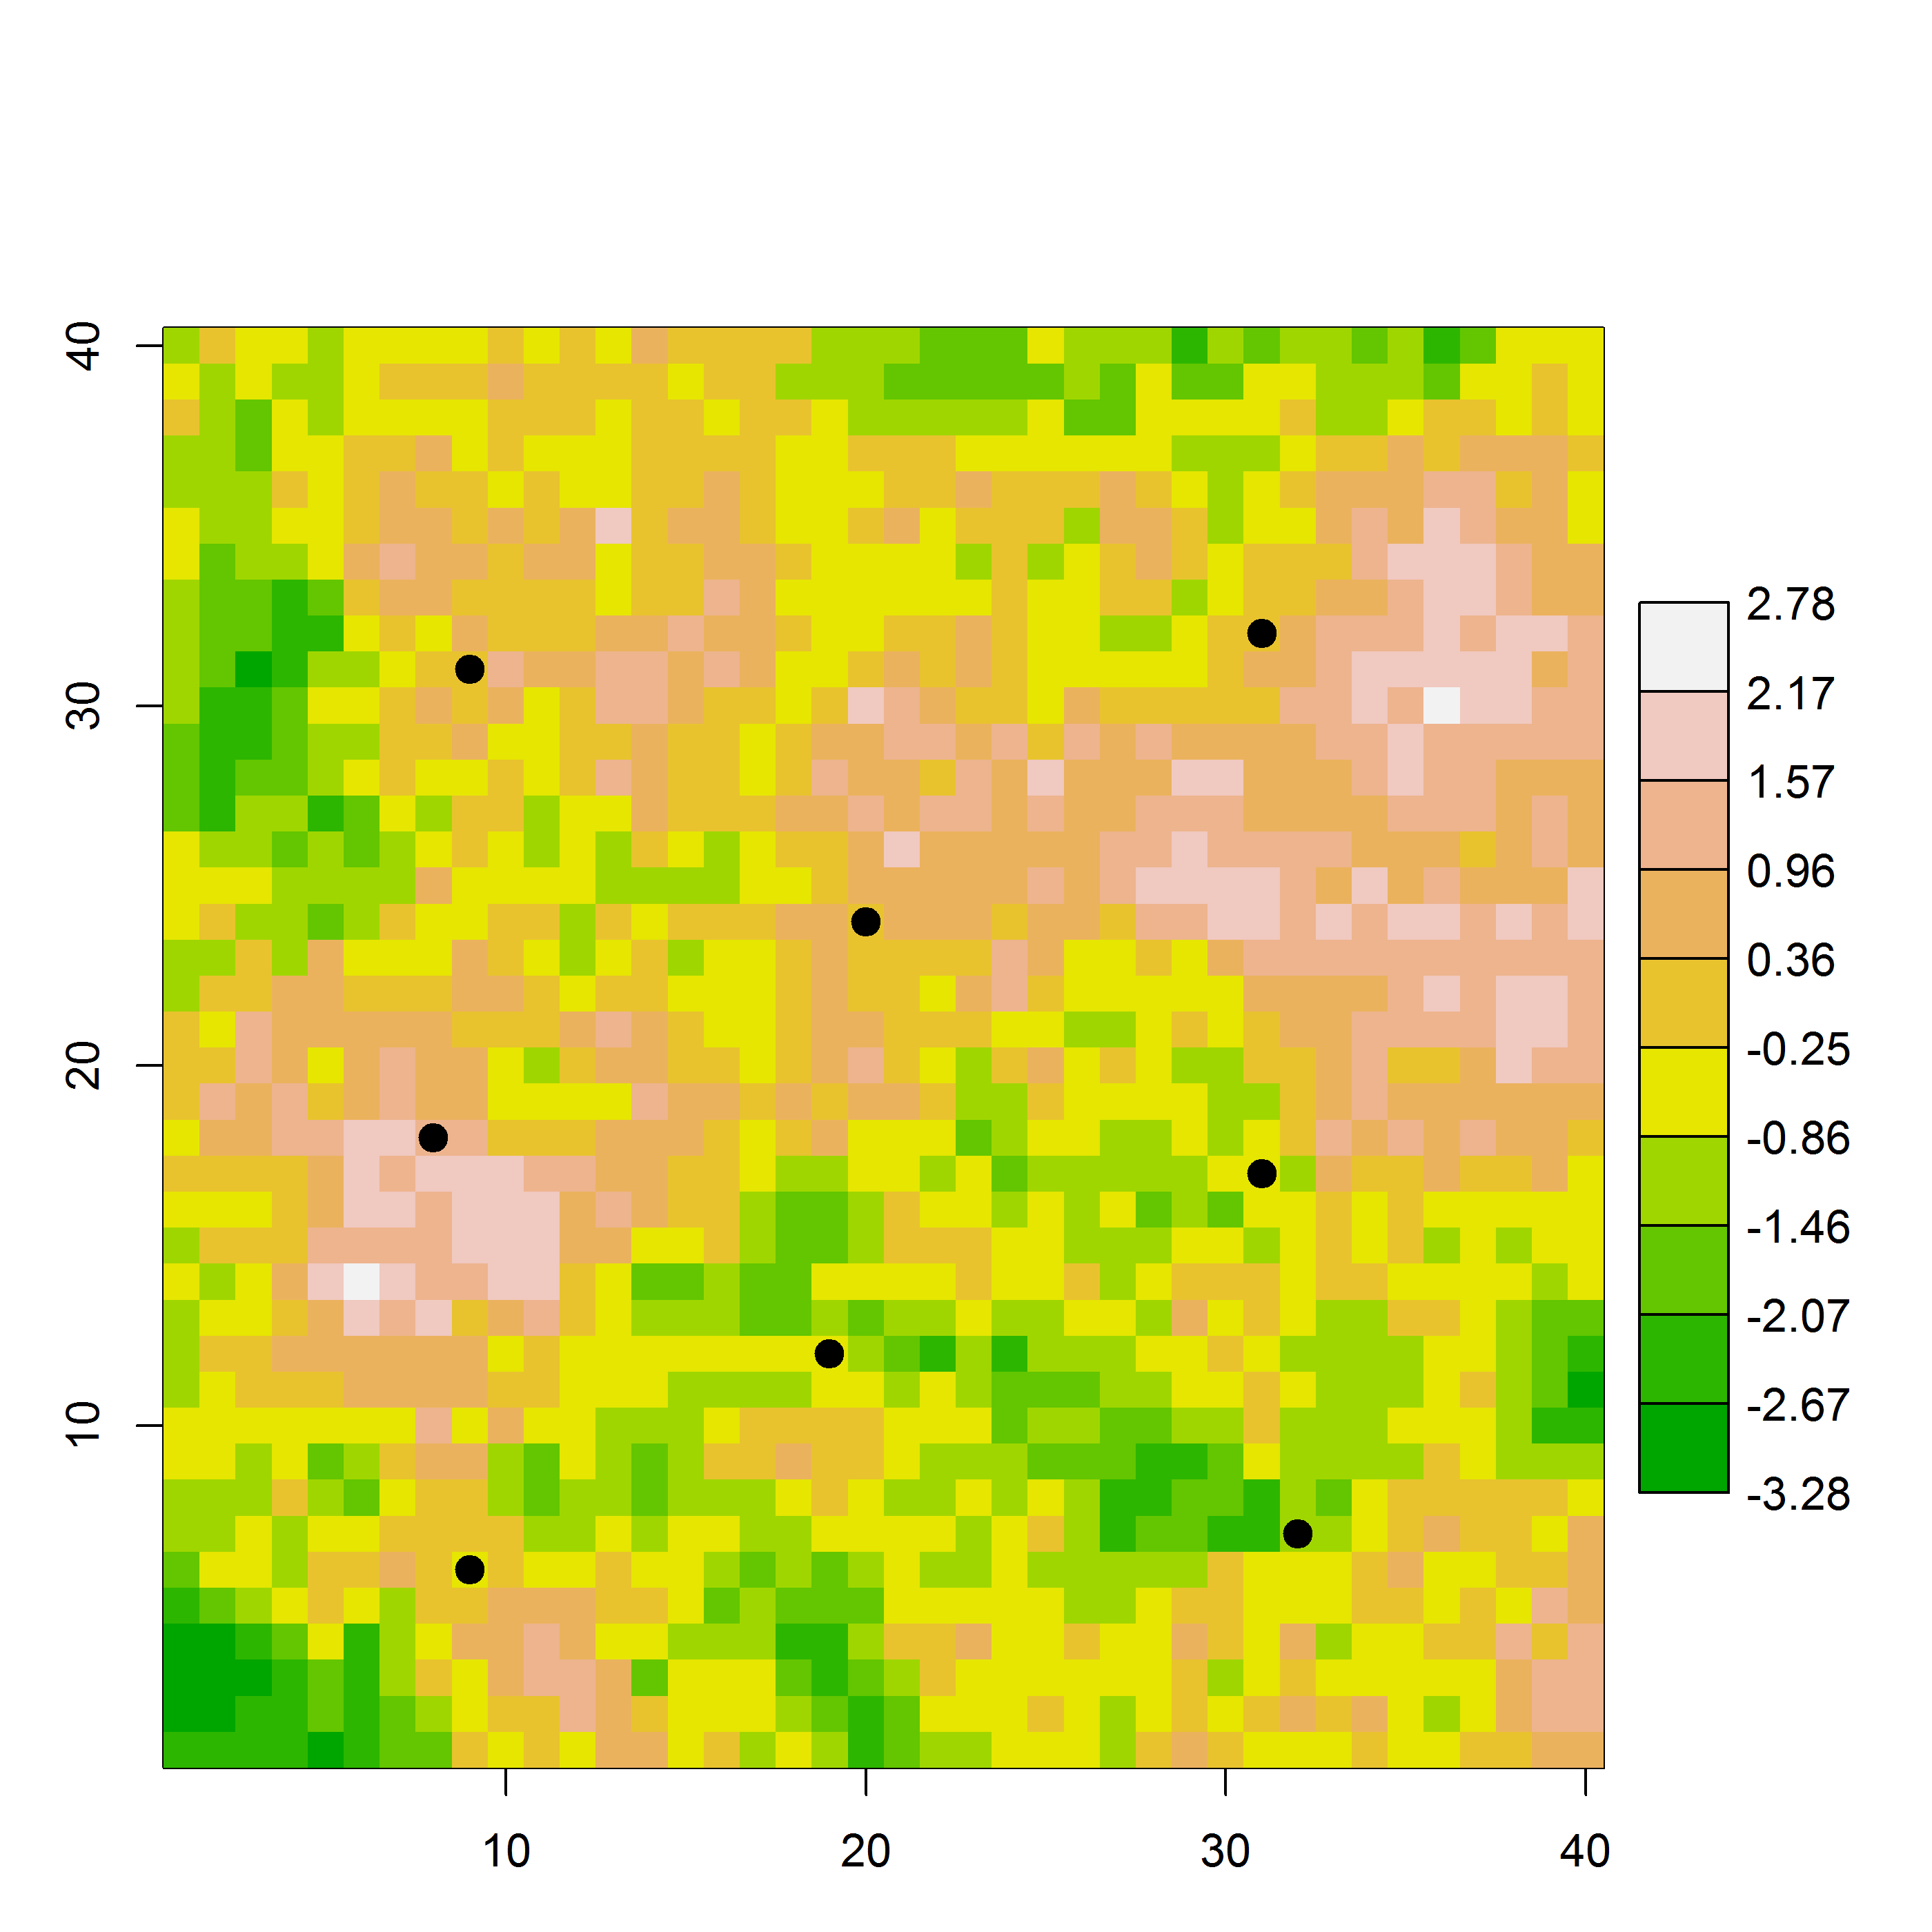
\includegraphics[width=3.15in,height=2.93in]{Ch13-RSF/figs/habitat.png}
\caption{A typical habitat covariate reflecting habitat quality or
  hypothetical utility of the landscape to a species under study. Home
  range centers for 8 individuals are shown with black dots.}
\label{rsf.fig.habitat}
\end{figure}

For a simulated landscape (shown in Fig. \ref{rsf.fig.habitat}),
\citet{royle_etal:2012mee} depicted some typical space
usage patterns under the model described above, which we reproduce
here in Fig.~\ref{rsf.fig.homeranges}.
\begin{figure}[ht]
\centering
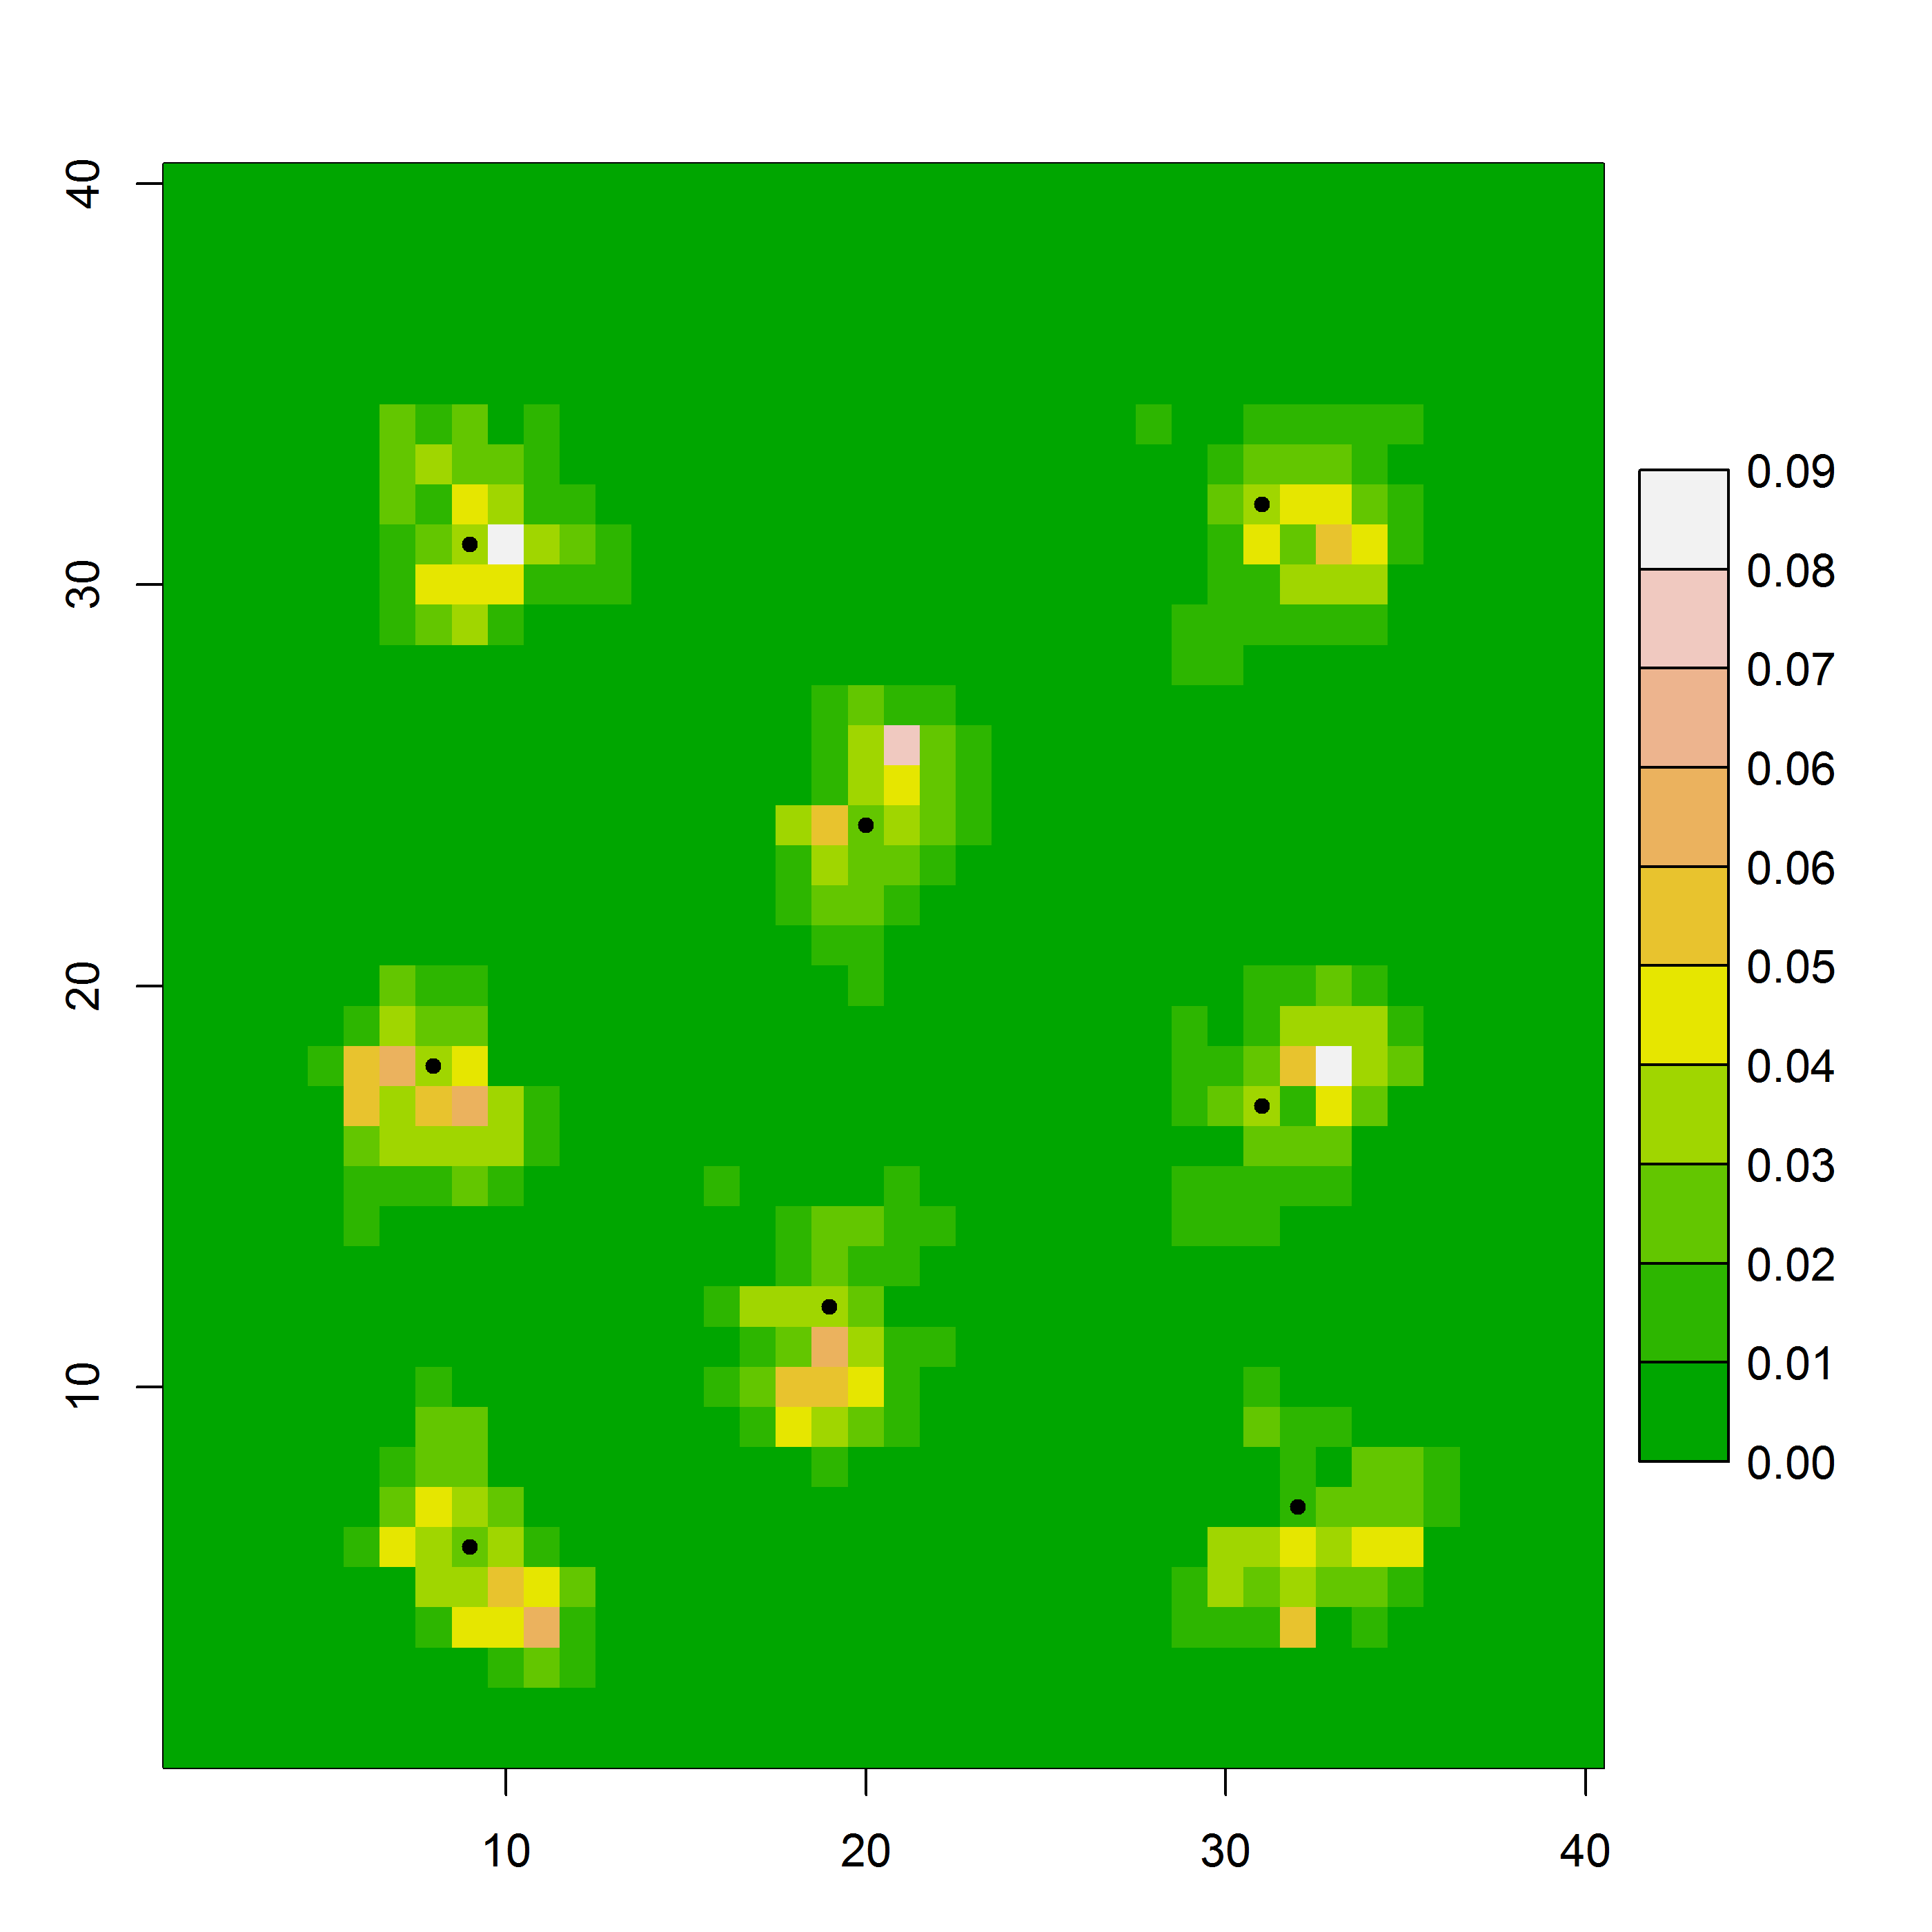
\includegraphics[width=3.5in,height=3.5in]{Ch13-RSF/figs/homeranges8}
\caption{Space usage patterns of 8 individuals under a space usage
  model that contains a single covariate which is shown in
  Fig. \ref{rsf.fig.habitat}. The plotted value is the multinomial
  probability $\pi_{ij}$ for pixel $j$ under the model in Eq. \ref{rsf.eq.rsf}.
}
\label{rsf.fig.homeranges}
\end{figure}
The covariate in this case was simulated using a kriging
model of correlated random noise
with the following {\bf R} commands:
\begin{verbatim}
> set.seed(1234)
> gr <- expand.grid(1:40,1:40)
> Dmat<-as.matrix(dist(gr))
> V <- exp(-Dmat/5)
> C <- t(chol(V))%*%rnorm(1600)
\end{verbatim}
The resulting covariate vector ${\bf C}$ is multivariate normal with
mean 0 and variance-covariate matrix ${\bf V}$ which, here, has
pairwise correlations which decay exponentially with distance.  The
use densities shown in Fig.~\ref{rsf.fig.homeranges} were simulated
with $\alpha_{1} = 1/(2\sigma^2)$, with $\sigma = 2$, and the
coefficient on $C({\bf x})$ set to $\alpha_{2} = 1$. The resulting
space usage densities -- or ``home ranges'' -- exhibit clear
non-stationarity in response to the structure of the underlying
covariate, and they are distinctly asymmetrical.  We note that if
$\alpha_{2}$ were set to 0, the 8 home ranges shown here would be
proportional to a bivariate normal kernel with $\sigma =
2$\footnote{This is why we have always referred to the similar-looking
  model for encounter probability as the Gaussian or bivariate normal
  model, instead of half-normal.}.  The commands for the kriging
model, and those to produce Fig. \ref{rsf.fig.habitat} are in the
package \mbox{\tt scrbook} (see \mbox{\tt ?RSF$\_$example}).


\subsection{Poisson model of space use}

A natural way to motivate the multinomial model of space usage is to
assume that individuals make a sequence of resource selection
decisions so that the outcomes $m_{ij}$ are {\it
  independent} Poisson random variables:
\[
 m_{ij} \sim \mbox{Poisson}( \lambda_{ij})
\]
where
\[
 \log(\lambda_{ij}) = a_{0} -\alpha_{1} d_{ij}^{2} +  \alpha_{2} C({\bf x}_{j})
\]
In this case, the number of visits to any particular cell is affected
by the covariate $C({\bf x})$ but has a baseline rate, $\exp(a_{0})$,
related to the amount (in an expected value sense) of movement occurring over some time interval.
This is an equivalent model to the multinomial model given previously
in the sense that, if we condition on the total sample size $R =
\sum_{j} m_{ij}$, then the vector ${\bf m}_{i}$ has a multinomial
distribution with probabilities given by Eq. \ref{rsf.eq.rsf} (see
also Chapt. \ref{chapt.poisson-mn}).

In practice, we never observe ``truth'', i.e., the actual use
frequencies $m_{ij}$. Instead, we observe a sample of the actual use
outcomes by an individual.  As formulated in
Sec.~\ref{scr0.sec.implied}, we assume a binomial (``random'')
sampling model:
\[
 y_{ij} \sim \mbox{Binomial}(m_{ij}, p_{0}).
\]
We can think of these counts as arising by thinning the underlying
point process (here, aggregated into pixels) where $p_{0}$ is the
thinning rate of the point process.  In this case, the marginal
distribution of the observed counts $y_{ij}$ is also Poisson but with
mean
\[
 \log(\mathbb{E}(y_{ij}))  = \log(p_{0}) + a_{0} -\alpha_{1} d_{ij}^{2} +  \alpha_{2} C({\bf x}_{j}).
\]
Thus, the space-usage model (RSF) for the thinned counts $y_{ij}$ is
the same as the space-usage model for the original variables $m_{ij}$.
This is because if we remove $m_{ij}$ from the conditional model by
summing over its possible values, then the vector ${\bf y}_{i}$ is
{\it also} multinomial with cell probabilities
\[
\pi_{ij} = \frac{\lambda_{ij}}{\sum_{j} \lambda_{ij}}
\]
where any constant (the intercept term $a_0$ and thinning rate
$p_{0}$) cancel from the numerator and denominator. Thus, the
underlying multinomial RSF model applies to the true unobserved count
frequencies ${\bf m}_{i}$ and also those produced from thinning or
sampling, ${\bf y}_{i}$.


\section{Integrating Capture-Recapture Data}

The key to combing RSF data with SCR data is to note that the Poisson
model of space usage given above is exactly our Poisson encounter
probability model from Chapt. \ref{chapt.poisson-mn}, only with a
spatial covariate $C({\bf x})$, and some arbitrary intercept off-set
related to the sampling rate by the telemetry device.  We've used
exactly this model for our SCR data (Chapt. \ref{chapt.covariates}),
but with a different intercept, $\alpha_{0}$, unrelated to the
intercept of the Poisson use model for telemetry described above but,
rather, to the efficiency of the capture-recapture encounter device.
In other words, we view camera traps (or other devices) located in
some pixel ${\bf x}$ (or multiple pixels) as being equivalent to being
able to turn on a type of (less perfect) telemetry device only in that
pixel.
Therefore,
data from a camera trapping are Poisson random variables
for every pixel $j$ where a trap is located:
\[
y_{ij}|{\bf s}_{i} \sim \mbox{Poisson}( \lambda_{ij})
\]
with
\[
 \log(\lambda_{ij}) =  \alpha_{0} -\alpha_{1}
 d_{ij}^{2} +  \alpha_{2} C({\bf x}_{j}).
\]
The parameters $\alpha_{1}$ and $\alpha_{2}$ are shared with the
multinomial model for the telemetry data.

Alternatively,
the SCR study can produce binary
encounters depending on the type of sampling being done,
where $y_{ij} = 1$ if the individual $i$ visited
the pixel containing a trap and was detected, then we imagine that
$y_{ij}$ is related to the latent variable $m_{ij}$ being the event
$m_{ij}>0$, which occurs with probability
\begin{equation}
 p_{ij} = 1-\exp(- \lambda_{ij})
\label{rsf.eq.cloglog}
\end{equation}
and then the observed encounter frequencies for individual $i$ and trap $j$, from
sampling over $K$ occasions are binomial:
\[
 y_{ij}|{\bf s}_{i} \sim \mbox{Binomial}(K, p_{ij})
\]

A key point here is that if resource selection is happening, then it
appears as a covariate on encounter rate (or encounter
probability) in the same way as ordinary covariates which we discussed in
Chapt. \ref{chapt.covariates}.

%%% trying to avoid having singleton subsections
%%%\subsection{The Joint RSF/SCR Likelihood}

To construct the likelihood for SCR data when we have
direct information on space usage
from telemetry data, we regard the two samples (SCR and RSF) as
independent of one another, and we
 form the likelihood for each set of observations as a function
of the same underlying parameters. The joint likelihood then is the
product of the two components.

In particular, let ${\cal L}_{scr}(\alpha_{0}, \alpha_{1}, \alpha_{2}, N;{\bf y})$
be the likelihood for the SCR data in terms of the basic encounter
probability parameters and the total (unknown) population size $N$,
and let ${\cal L}_{rsf}(\alpha_{1},\alpha_{2}; {\bf m})$ be the
likelihood for the RSF data based on telemetry which, because the
sample size of telemetered individuals is fixed, does not depend on $N$.
Assuming independence of the two datasets, the
joint likelihood is the product of these two pieces:
\[
{\cal L}_{rsf+scr}(\alpha_{0},\alpha_{1},\alpha_{2},N; {\bf y},{\bf
  m})  =
{\cal L}_{scr}(\alpha_{0}, \alpha_{1}, \alpha_{2}, N;{\bf y})
\times
{\cal L}_{rsf}(\alpha_{1},\alpha_{2}; {\bf m}),
\]
where the ${\cal L}_{scr}$ is the standard integrated likelihood
(Chapt. \ref{chapt.mle}), and the RSF likelihood contribution is the
multinomial telemetry likelihood having cell probabilities
Eq. \ref{rsf.eq.rsf}.  The {\bf R} code for maximizing the joint likelihood
was given in the
supplement to \citet{royle_etal:2012mee}, and we include a version of
this in the \mbox{\tt scrbook} package, see \mbox{\tt ?intlik3rsf},
which also shows how to simulate data and fit the combined SCR+RSF
model.


\section{SW  New York Black Bear Study}
\label{rsf.chapt.nybears}

\citet{royle_etal:2012mee} applied the integrated SCR+RSF model to
data from a study of black bears ({\it Ursus americanus})
in a region of approximately 4,600
km$^2$ in southwestern New York.  These data come from a research
project by C. Sun \citep{sun:2013} at Cornell University, and it is a
different data set than our Fort Drum bear study data set which we've analyzed
in previous chapters.  The data can be loaded from the \mbox{\tt scrbook}
package with the command \mbox{\tt data(nybears)}.
We reproduce the findings of \citet{royle_etal:2012mee} in this section.

The data are based on a noninvasive genetic capture-recapture study
using 103 hair snares in June and July, 2011.  Hair snares were baited
and scented and checked weekly for hair \citep{sun:2013}.  The study
yielded relatively sparse encounter histories
 of 33 individuals with a total of 14 recaptures and 27
individuals captured 1 time only.
Telemetry data were collected on 3 telemetry-collared individuals, which produced
locations for each bear approximately once per hour.  Telemetry
locations were
thinned to once per 10 hours to produce movement outcomes that might
be more independent. This produced 195 telemetry locations used in the
RSF component of the model.  Elevation was used as the covariate for this
model, a standardized version of which is shown in
Fig. \ref{fig.elevation} along with the locations of each
capture at hair snare sites.


\begin{figure}[ht]
\centering
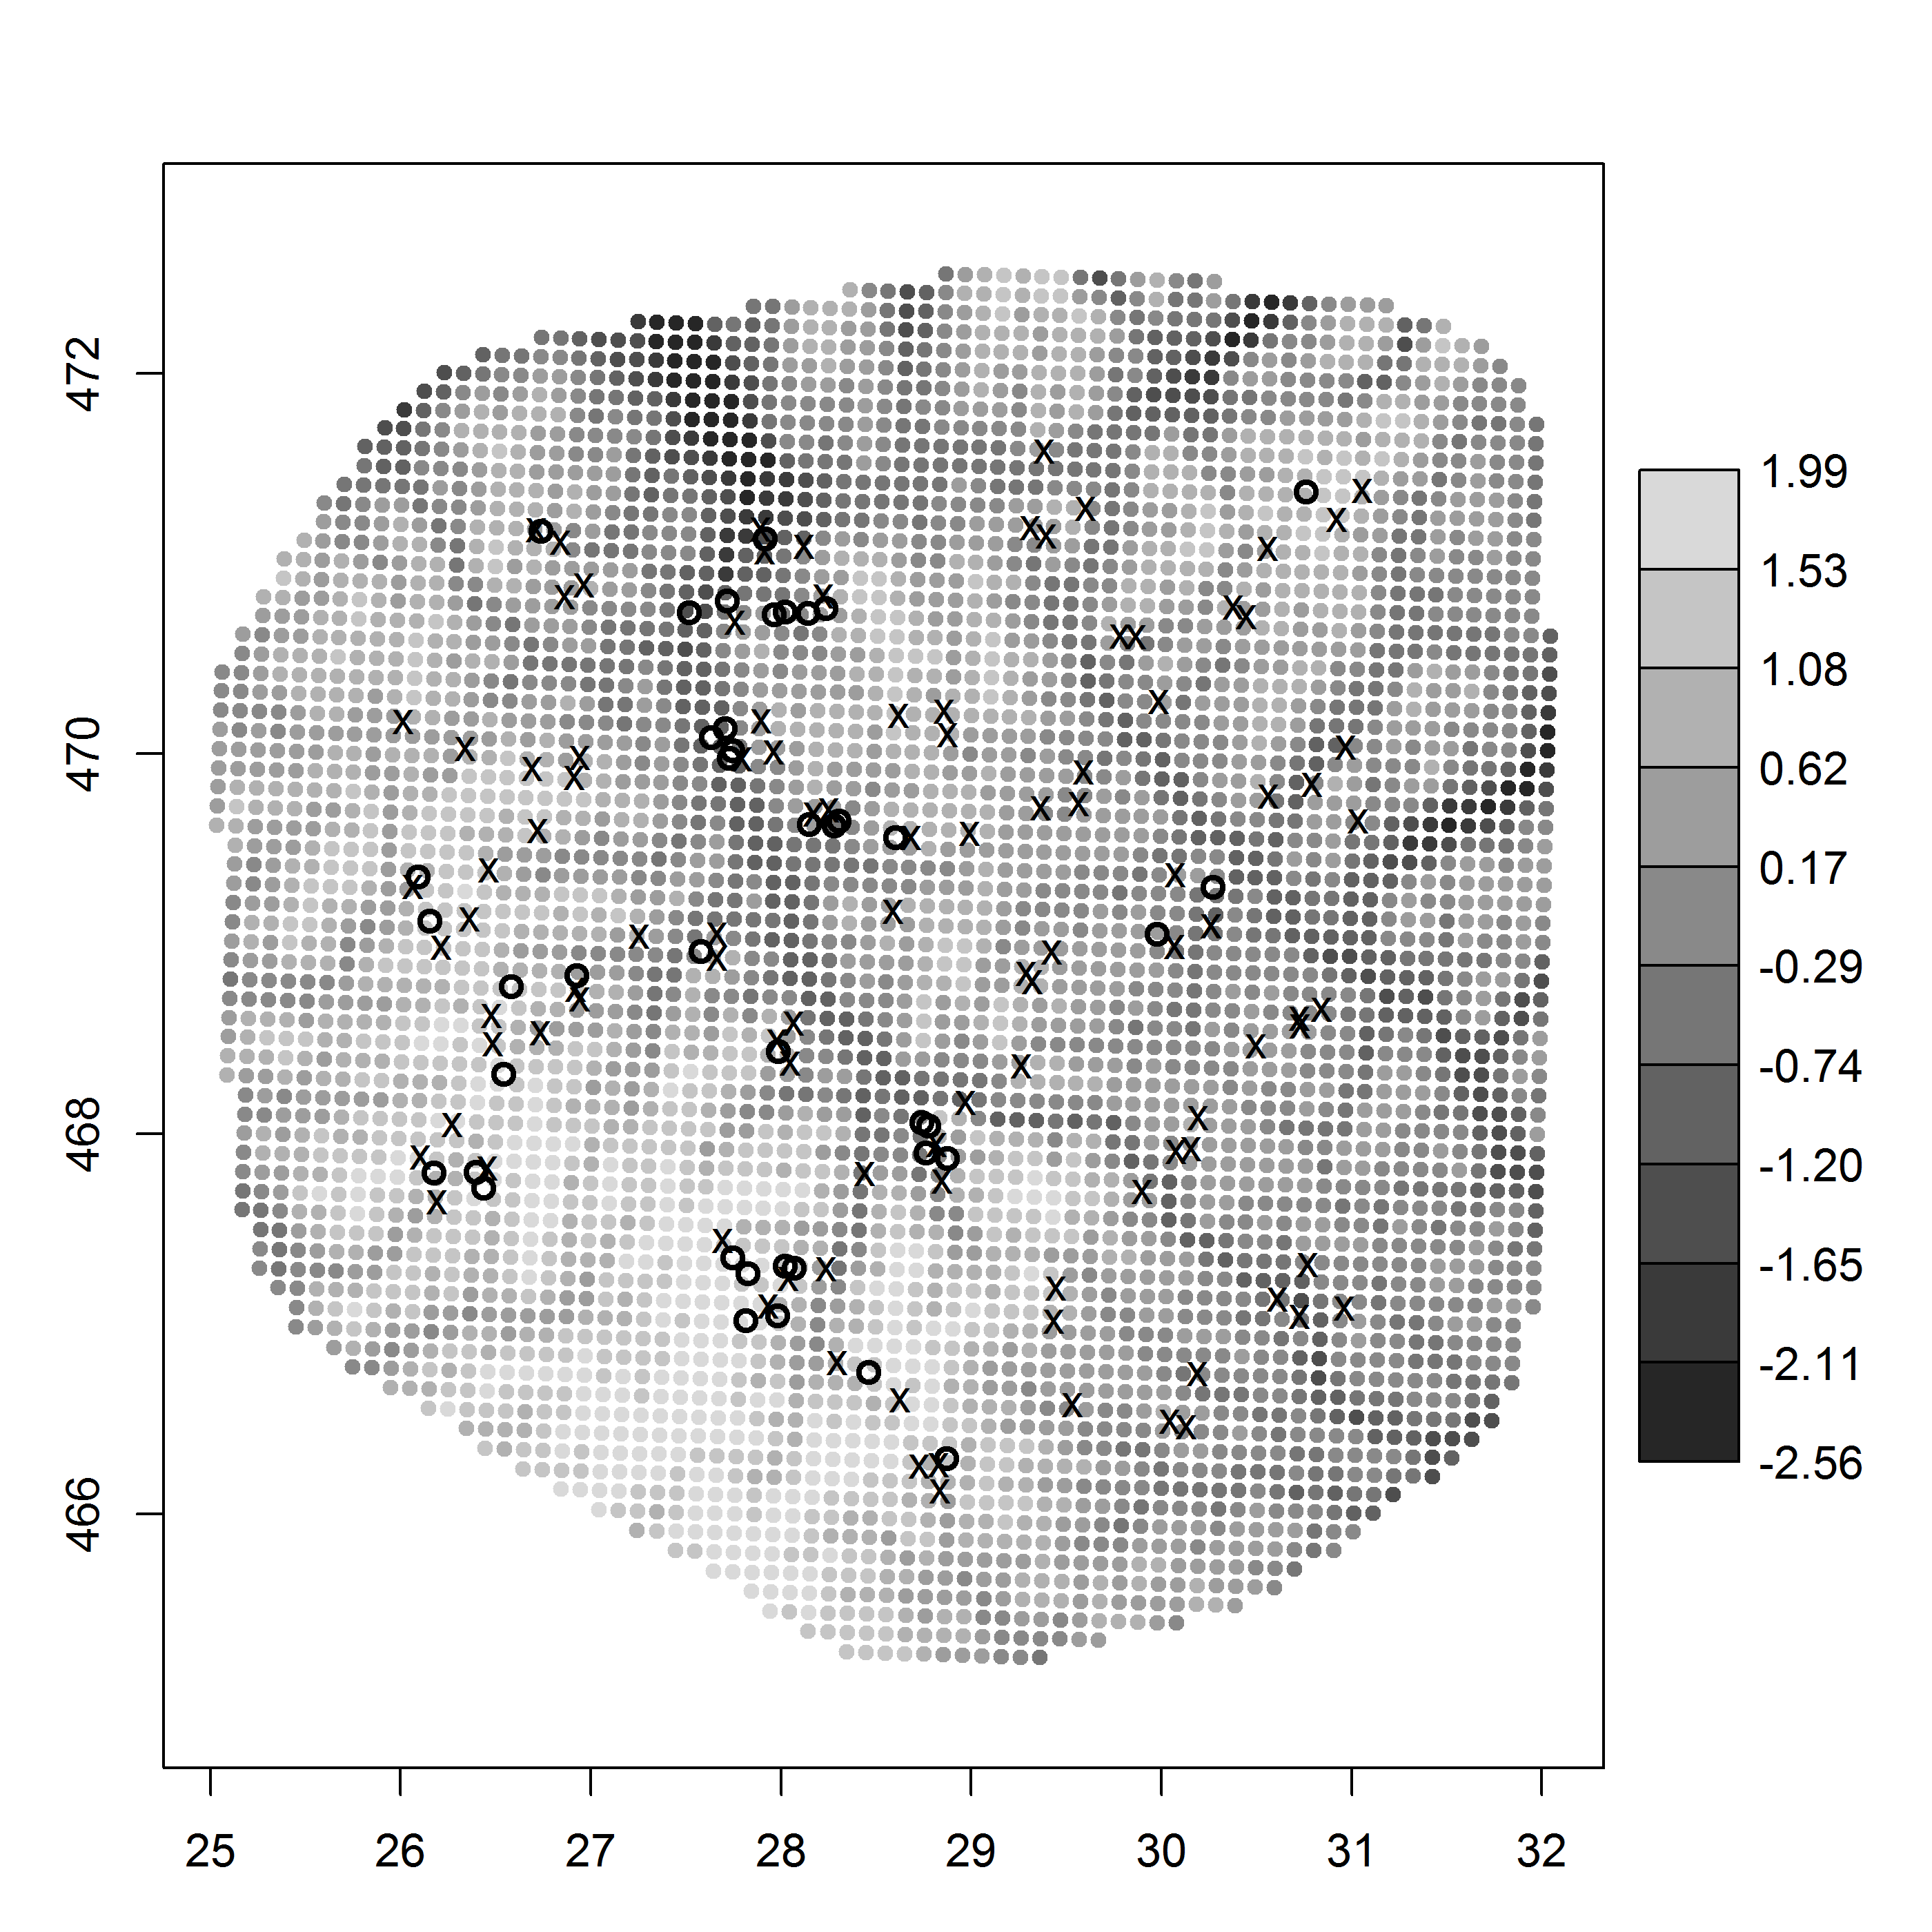
\includegraphics[width=3.25in,height=3.25in]{Ch13-RSF/figs/elev_captures_bw.png}
\caption{
Elevation (standardized), hair snare locations (indicated by ``x'') and location
of bear captures (open circles).
Multiple captures at a trap location are offset from the hair snare
sites by adding
random noise.
}
\label{fig.elevation}
\end{figure}

%XXXX RS: I think this figure needs some work; symbols are difficult to distinguish. XXXX

There are a number of models that could be fitted to these data based on
the combination of SCR and RSF data as well as the elevation covariate.
The models fit here are
 based on the Gaussian hazard trap encounter/space usage model,
including an ordinary SCR model with no covariates or telemetry data,
the SCR model with elevation affecting either $\lambda_{0}$ or density
$D({\bf x})$ (Chapt. \ref{chapt.state-space}), and models that use
telemetry data.  The 6 models fitted were:
\begin{itemize}
\item[] Model 1, SCR: ordinary SCR model

\item[] Model 2, SCR+p(C): ordinary SCR model with elevation as a
  covariate on baseline encounter probability $\lambda_{0}$.

\item[] Model 3, SCR+D(C): ordinary SCR model with elevation as a
  covariate on density only.

\item[] Model 4, SCR+p(C)+D(C): ordinary SCR model with elevation as
  a covariate on both baseline encounter probability and density.

\item[] Model 5, SCR+p(C)+RSF: SCR model including data from 3
  telemetered individuals.

\item[] Model 6, SCR+p(C)+RSF+D(C): SCR model including telemetered
  individuals and with elevation as a covariate on density.
\end{itemize}
Parameter estimates for the six models are
given in Table \ref{tab.nyresults} (reproduced from
\citet{royle_etal:2012mee}, see also the help file \mbox{\tt
  ?nybears}).
It is tempting to want to compare these different models by AIC but,
because models 5 and 6 involve additional data, they cannot be
compared with models 1-4.

By looking at Table \ref{tab.nyresults}, it is clear based on the
negative log likelihood for just Models 1-4, that those containing an
elevation effect on density are preferred (Model 3 and 4).  The
parameter estimates indicate a positive effect of elevation on
density, which seems to be consistent with the raw capture data shown
in Fig. \ref{fig.elevation}.  Despite this strong effect
of elevation, the estimates of $N$ under each of these models only
ranged from $93 - 103$ bears for the 4600 km$^2$ state-space, and so
estimated density is pretty consistent across models.
  If we
consider not just density, but space usage (i.e., looking at the
parameter $\alpha_2$), the effect of elevation is negative.  Thus, elevation, appears to affect density and space usage
differently.  It was suggested that density operates at the
second-order scale of resource selection and ``....is largely related
to the spacing of individuals and their associated home ranges across
the landscape.  On the other hand, our RSF was defined based on
selection of resources within the home range (third-order).''
\citep{royle_etal:2012mee}
The positive effect of density on elevation
is consistent with some other studies on black bears \citep[e.g.][]{frary_etal:2011},
and the negative effect of elevation on space usage can be attributed to
seasonal variation in food availability, usage of corridors, or
environmental conditions.


Models 5 and 6 include the additional telemetry data, thus the
negative log-likelihoods are not directly comparable to the first 4
models, but we can still make a few important observations.  First is
that the parameter estimates under these two models are consistent
with Model 4 in that elevation had a strong effect on both density and
space usage.  In comparing models 5 and 6, the latter model which
includes elevation as an effect on density reduces the negative
log-likelihood by 5 units.  Additionally, including the telemetry data
reduces the standard errors (SE) of the density and space usage
parameters and as we would expect, the incorporation of telemetry data
also reduces the SE for $\sigma$.  The increased precision for the
estimated population size ($N$) is negligible with the use of
telemetry data in this case.  However, that may be different if more
telemetry information were available.  Model 6 (SCR+p(C)+RSF+D(C)),
was used to produce maps of density (Fig. \ref{fig.density}) and space
usage (Fig. \ref{fig.spaceusage}) showing the effect of elevation on
both components of the model.  The map of space usage shows the
relative probability of using a pixel ${\bf x}$ relative to one having
the mean elevation, given a constant distance to the individual's
activity center.


\begin{table}
\centering
\caption{
Summary of model-fitting results for the black bear study. Parameter
estimates are for the intercept ($\alpha_{0}$), logarithm of $\sigma$,
the
scale parameter of the Gaussian hazard encounter model,
 $\beta$ is the coefficient of elevation on density, and the total
 population size $N$ of the state-space. Standard errors
 are in parentheses.
The SCR data are based on $n=33$ individuals, and the telemetry data
are based on 3 individuals.
}
\begin{tabular}{c|rrrrrr}
\hline \hline
model         & $\alpha_0$ & $\log(\sigma)$ & $\alpha_{2}$ & $N$ &
$\beta$       & -loglik                                                                         \\ \hline
SCR(elev)      & -2.860    & -1.117        & 0.175       & 95.8        &        & 122.738  \\
             &  (0.390)     & (0.139)       & (0.248)       & (22.99)        &        &           \\
SCR          & -2.729    & -1.122        & ---          & 93.9        &        & 122.990  \\
              & (0.345)     & (0.140)       &              & (22.06)        &        &           \\
SCR+D(elev)      & -2.715    & -1.133        & ---          & 94.2        & 1.247 & 118.007  \\
              & (0.353)     & (0.139)       &              & (21.90)    & (0.408) &           \\
SCR(elev)+D(elev) & -2.484    & -1.157        & -0.384      & 103.5        & 1.571 & 117.075  \\
              & (0.391)     & (0.142)       & (0.276)       & (26.56)   & (0.463) &           \\
SCR(elev)+RSF       & -3.068    & -0.814        & -0.281      & 81.6        &        & 1271.739 \\
              & (0.272)    & (0.036)         & (0.118)       & (17.65)        &        &           \\
SCR(elev)+RSF+D(elev)  & -3.070    & -0.810        & -0.371      & 89.1        & 1.273 & 1266.700 \\
              & (0.272)    & (0.037)         & (0.124)       & (20.55)        & (0.411) &           \\
\hline
\end{tabular}
\label{tab.nyresults}
\end{table}



\begin{figure}
\centering
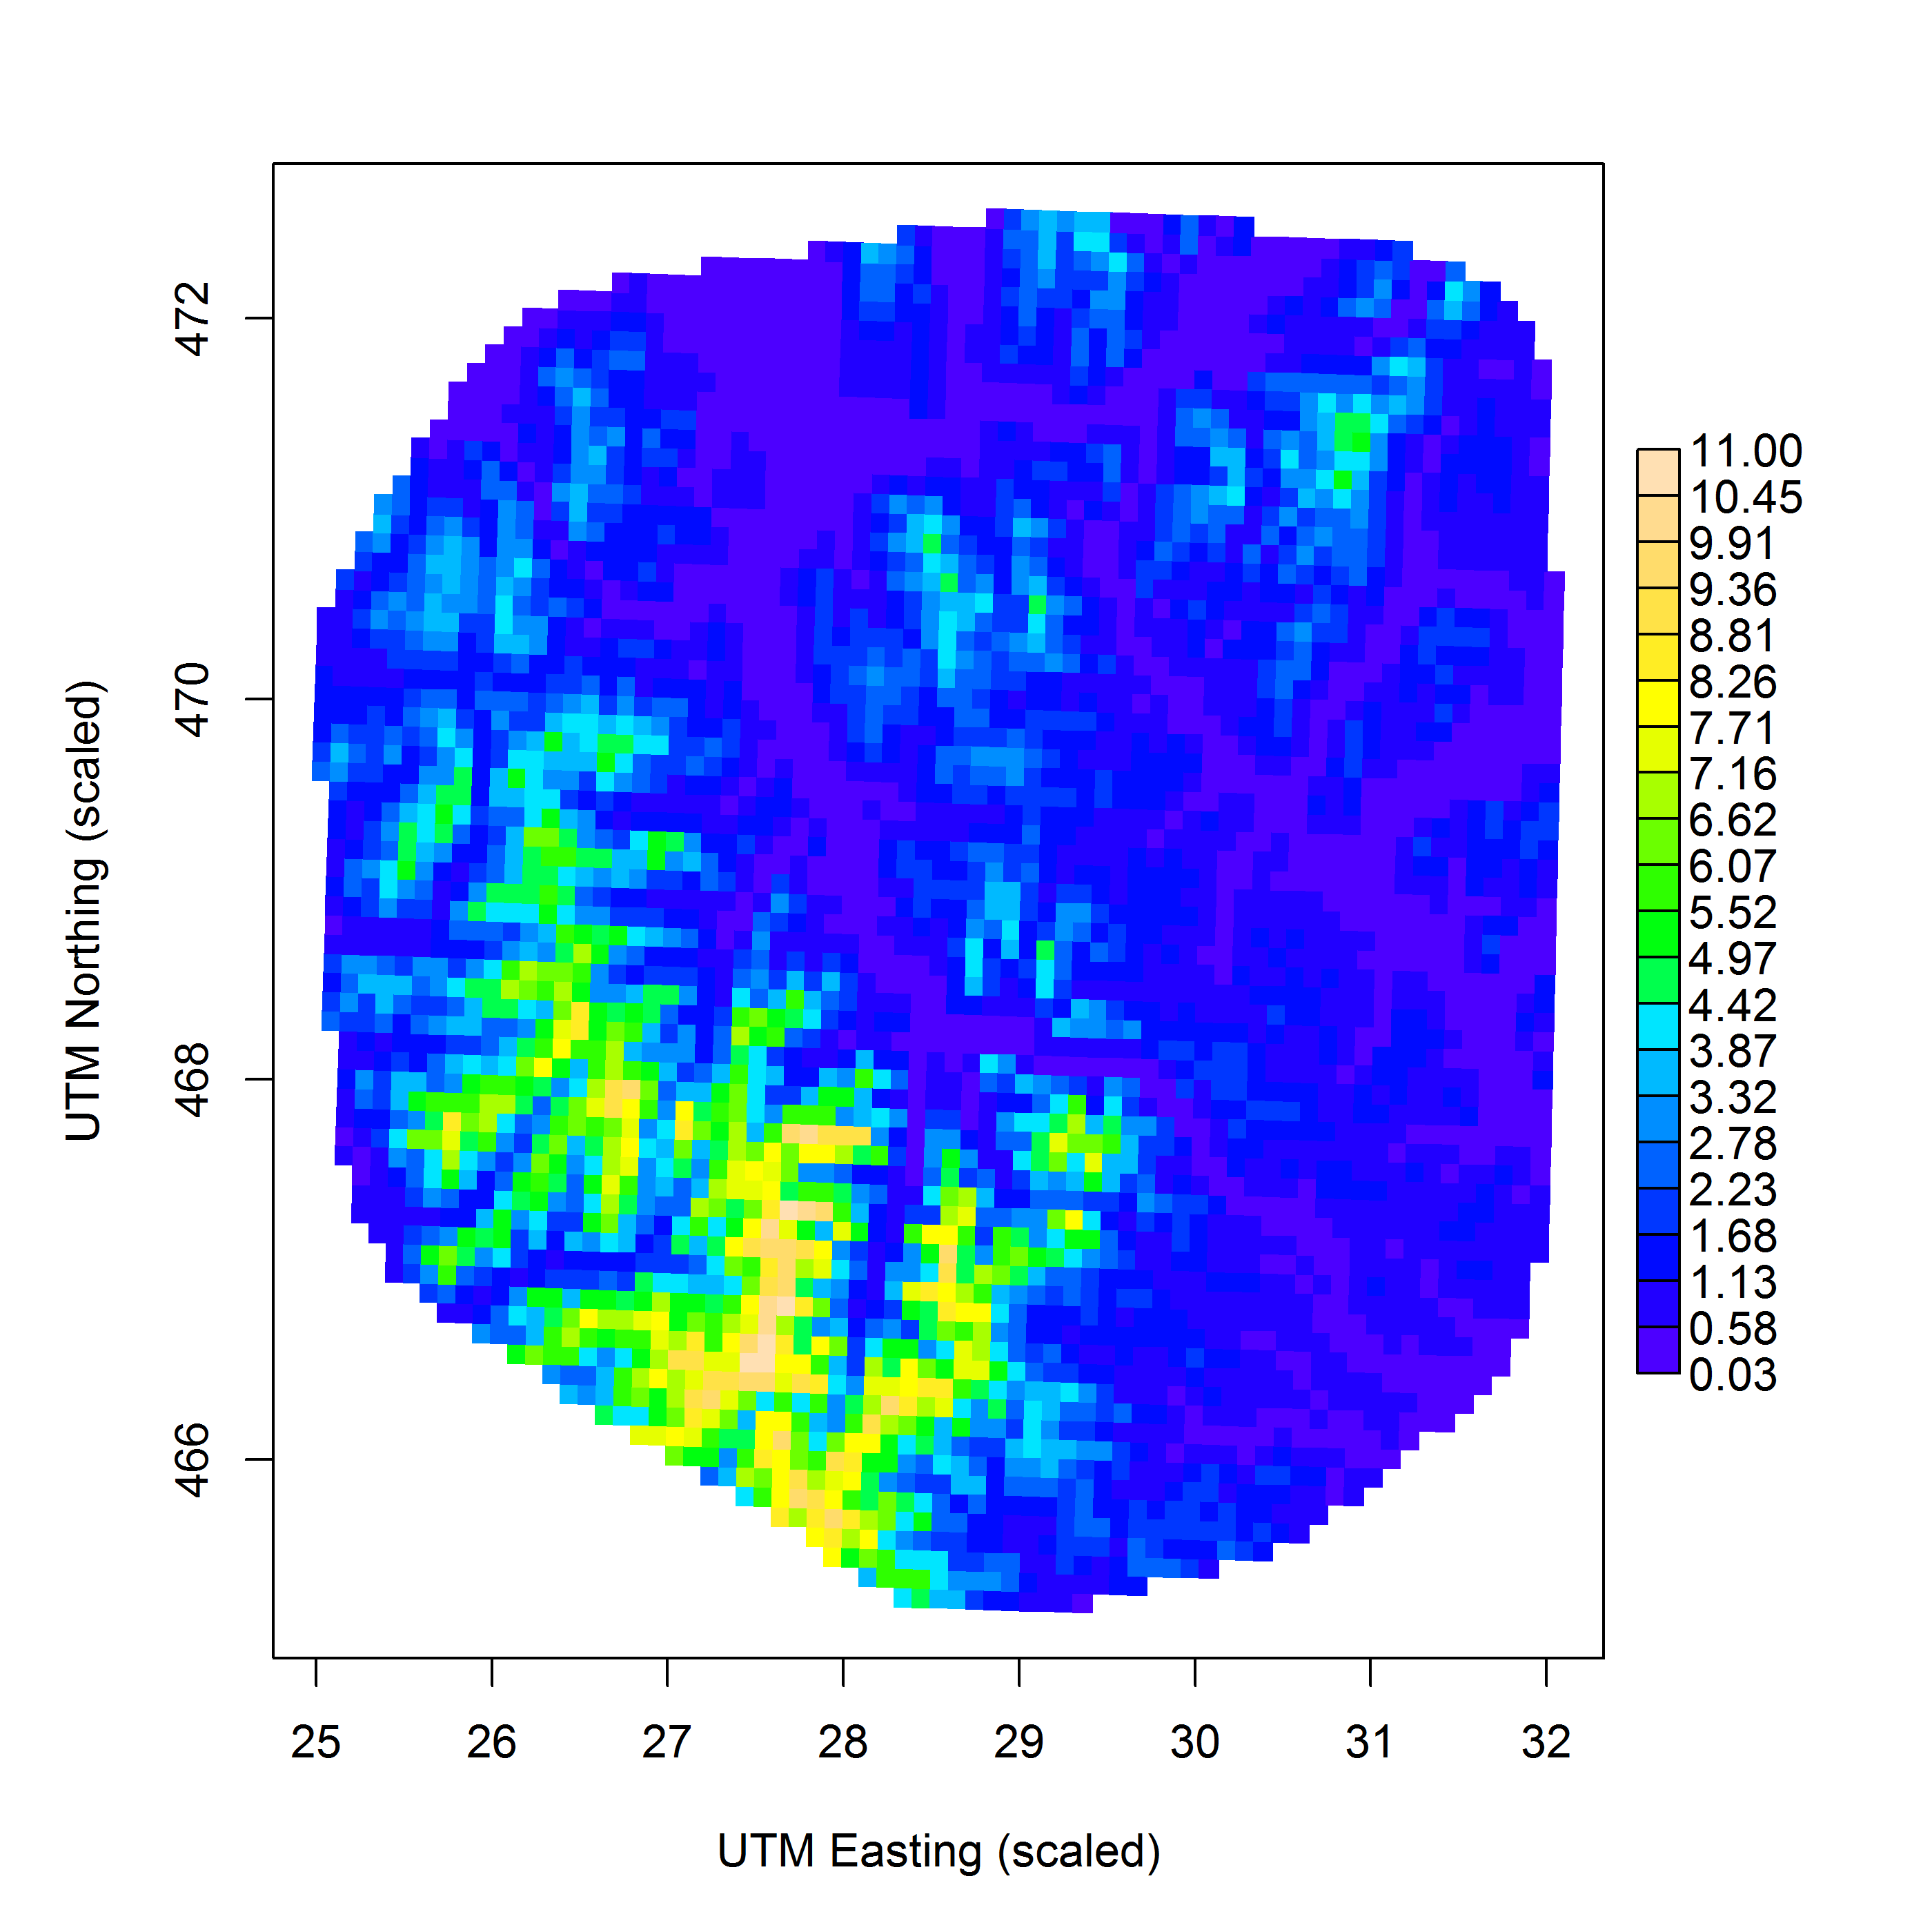
\includegraphics[width=3.25in,height=3.25in]{Ch13-RSF/figs/density2.png}
\caption{Predicted density of black bears (per 100 km$^2$) in
  southwestern  New York study
  area.
}
\label{fig.density}
\end{figure}


\begin{figure}
\centering
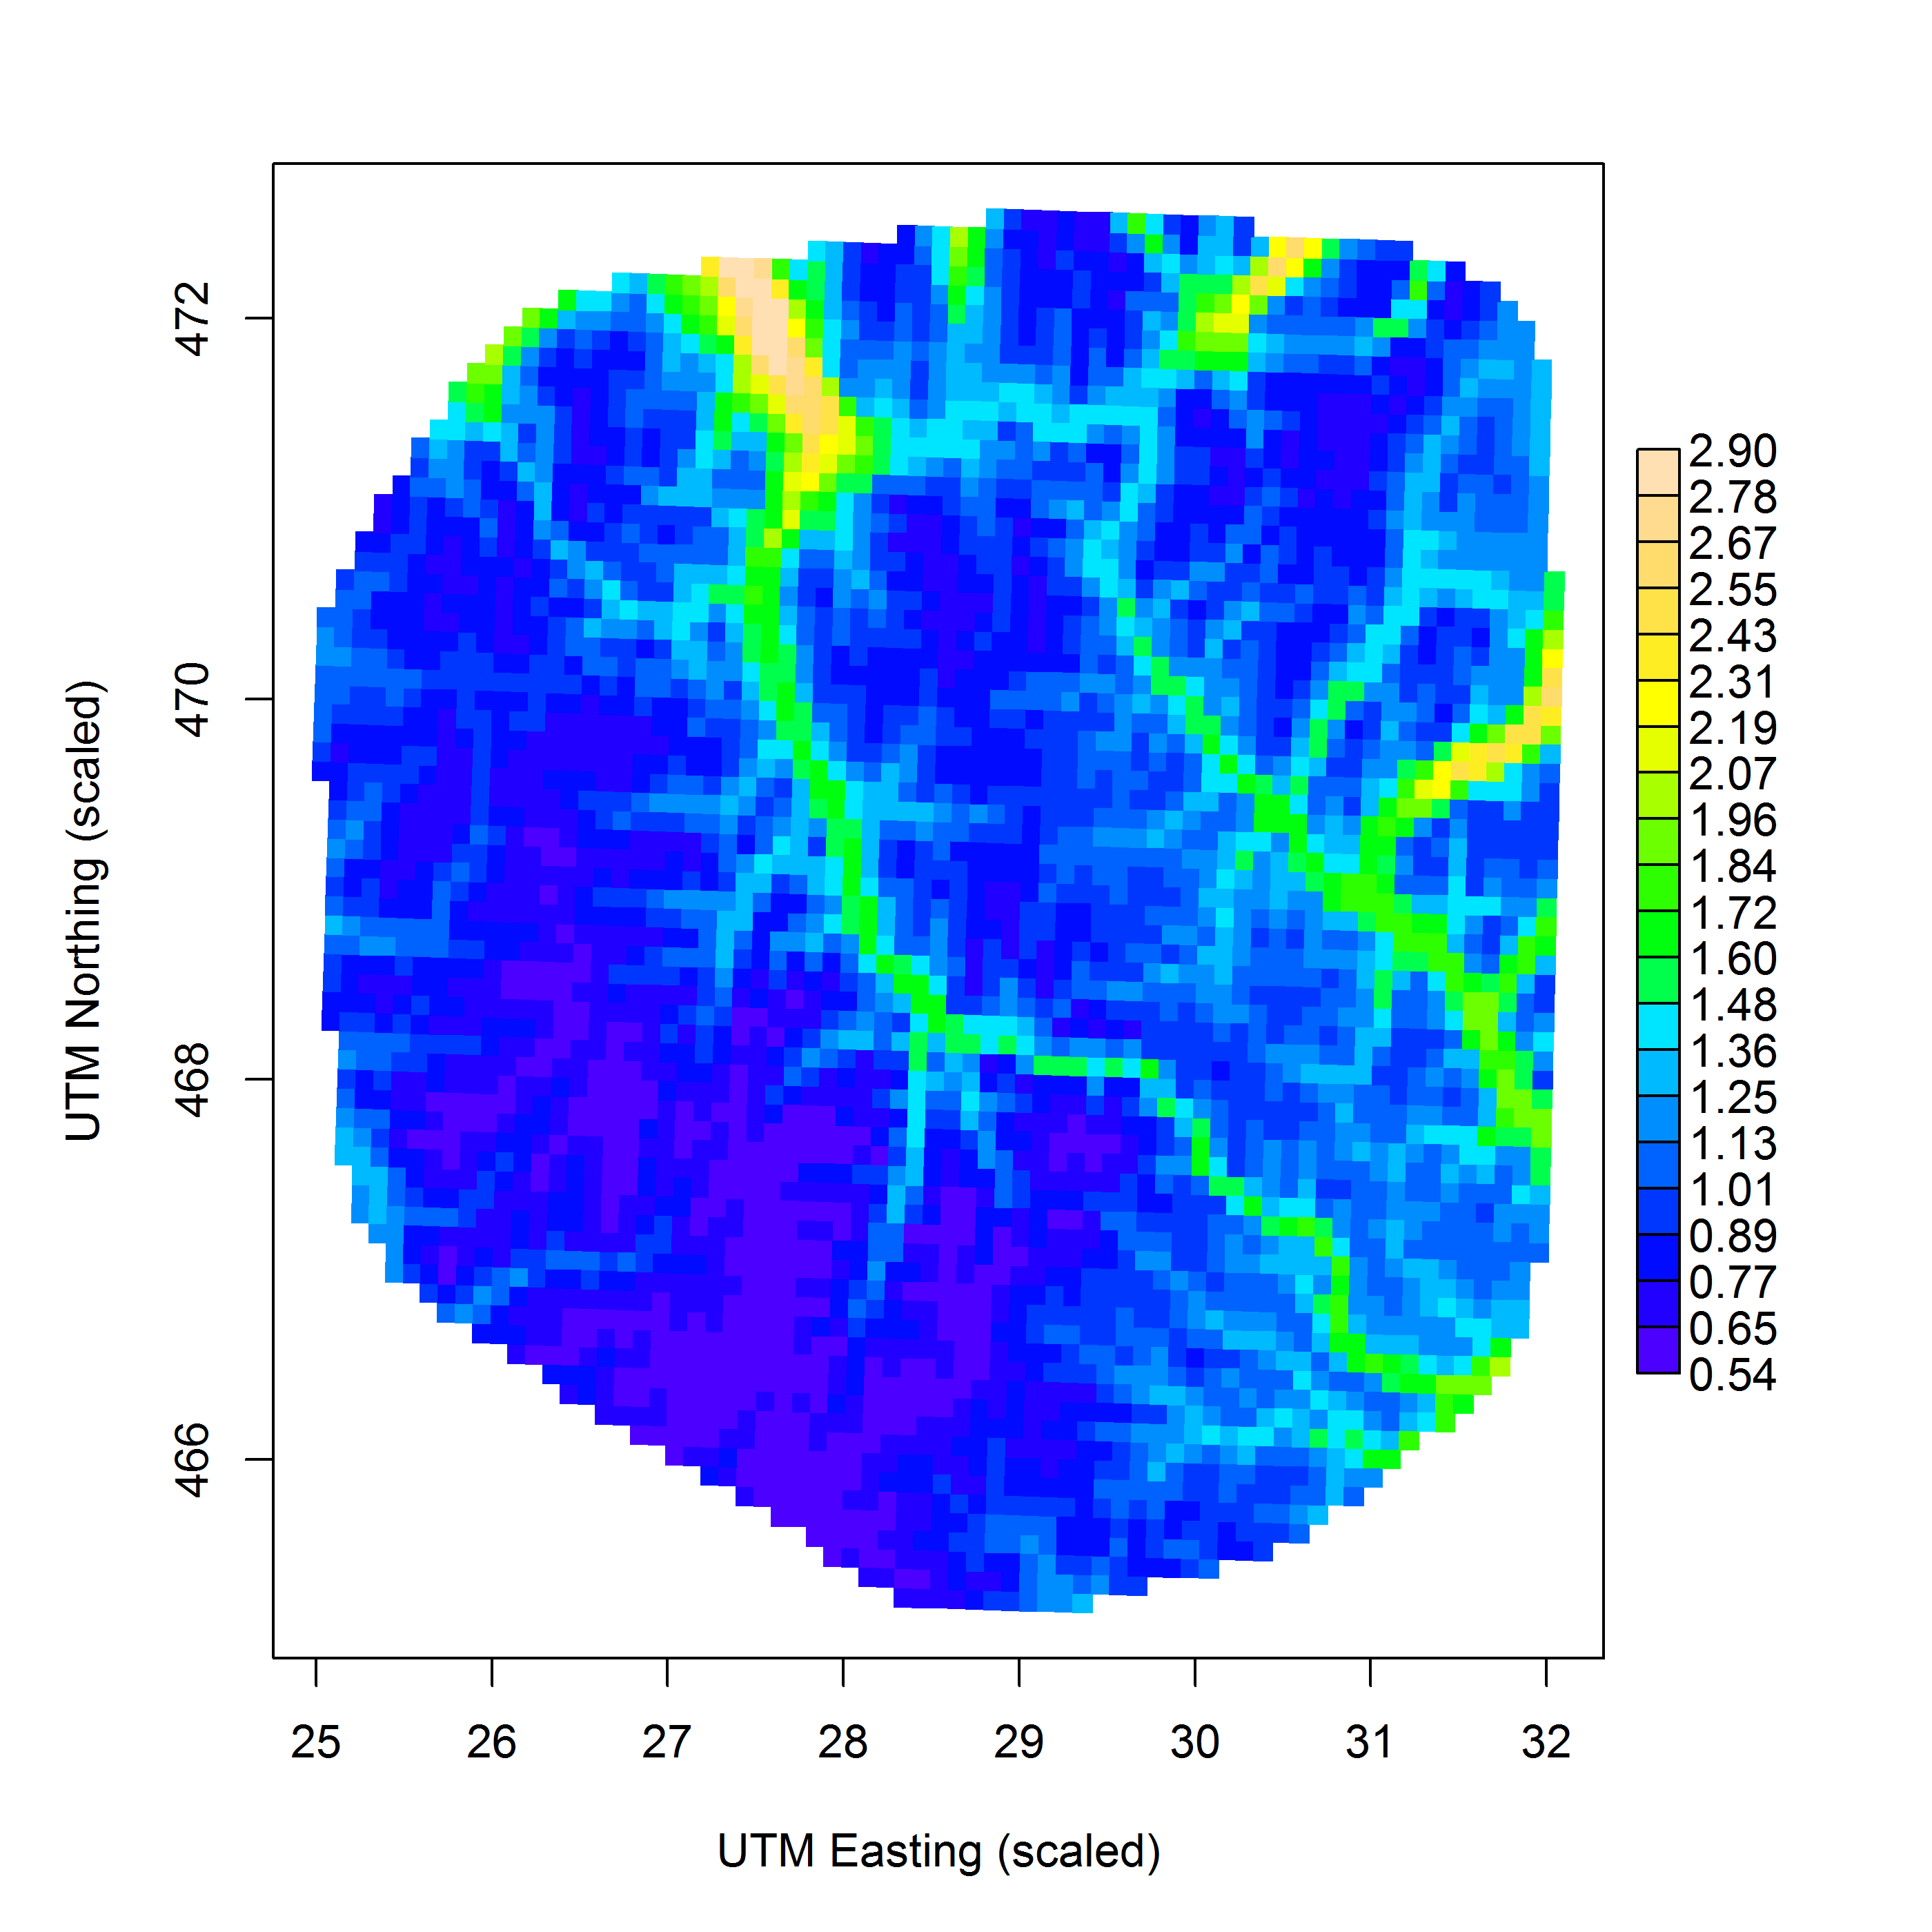
\includegraphics[width=3.25in,height=3.25in]{Ch13-RSF/figs/spaceusage2.png}
\caption{Relative probability of use of pixel ${\bf x}$ compared to a pixel
  of mean elevation, at a constant distance from the activity center.
}
\label{fig.spaceusage}
\end{figure}



\section{Simulation Study}

Using the simulated landscape shown in Fig. \ref{rsf.fig.habitat},
\citet{royle_etal:2012mee} presented results of a simulation study
considering populations of $N=100$ and $N=200$ individuals exposed to
encounter by a
 $7 \times 7$ array of trapping devices,
with $K=10$ sampling occasions, using
the Gaussian hazard model
(Eq. \ref{rsf.eq.cloglog})
with
\[
\log(\lambda_{ij}) = -2  -\frac{1}{2\sigma^{2}} d_{ij}^{2} + 1 * C({\bf x}_{j}).
\]
where $\sigma =2$.
They looked at the effect of misspecification of the resource
selection model with an ordinary model SCR0 (i.e. no habitat
covariates affecting the trap encounter model), and the performance of
the MLEs, under SCR+telemetry designs having 2, 4, 8, 12, and 16
telemetered individuals (with 20 independent telemetry fixes {\it per}
individual). Three models were fitted: (i) the SCR only model, in
which the telemetry data were not used; (ii) the integrated SCR/RSF
model which combined all of the data for jointly estimating model
parameters; and (iii) the RSF only model which just used the telemetry
data alone (and therefore the parameters $\alpha_{0}$ and $N$ are not
estimable).  An abbreviated version of the results from
\citet{royle_etal:2012mee} is summarized in Table \ref{rsf.tab.sims}.
We provide an {\bf R} script (see \mbox{\tt ?RSFsim}) that can
be modified for further analysis and exploration.

One thing we see is a pretty dramatic negative bias in estimating $N$
if the model SCR0 is fitted (interestingly, there is much less bias in
estimating $\sigma$).  Overall, though, when either the SCR model with
covariate or the joint SCR+RSF model is fitted, the MLEs exhibit
little bias for the parameter values simulated here. In terms of RMSE,
there is only a slight $\approx$ 5-10\% reduction in RMSE of the
estimator of $N$ when we have at least 2 telemetered individuals.
Thus, estimating $N$ benefits only slightly from the addition of
telemetry data, which is because information about the intercept,
$\alpha_{0}$, comes only from the capture-recapture data.  However,
there is a large improvement in precision (50-60\%) for estimating the
scale parameter $\sigma$.  While this doesn't translate much into
improved estimation of $N$, it suggests that it should be relevant to
the design of SCR studies for which trap spacing is one of the main
considerations (Chapt. \ref{chapt.design}). In terms of study design
these results also suggest that, perhaps, spatial recaptures are not
needed if some telemetry data are available (in
Chapt. \ref{chapt.partialID}, in the context of mark-resight models,
we show a case study of raccoons where additional telemetry data
allows estimating model parameters in spite of a very low number of
spatial recaptures \citep{sollmann_etal:2012ecol}). The resource
selection parameter $\alpha_{2}$ is well-estimated even {\it without}
telemetry data. The fact that parameters of resource selection can be
estimated from ordinary capture-recapture data should have
considerable practical relevance in the study of animal populations
and landscape ecology. For the highest sample size of telemetered
individuals ($n=16$), the RMSE for estimating this parameter only
decreases from about $0.09$ to $0.07$.


\begin{table}[ht]
\centering
\caption{
  This table summaries the sampling distribution of the MLE of model
  parameters   for models fitted to data generated under a resource selection model.  The models fitted   include the misspecified model, which is a basic model SCR0 (with no covariate), the SCR model with
  the covariate on encounter probability, and the SCR model including
  the covariate and a sample of telemetered individuals ($n$ is the
  number of individuals telemetered).    Data were simulated with   $N=200$ individuals,
  $\alpha_{2} = 1$ and $\sigma = 2$.
}
\begin{tabular}{ccccccc} \hline \hline
        &  $\hat{N}$ &RMSE   &  $\hat{\alpha}_{2}$ &RMSE  &        $\hat{\sigma}$ & RMSE    \\ \hline
n=2     &       &       &       &      &        &         \\
SCR+C(x)& 199.11&  14.28&  0.99 &  0.09&   2.00 &  0.090  \\
SCR+RSF & 199.11&  13.80&  0.99 &  0.09&   2.00 &  0.079  \\
SCR0    & 161.48&  39.98&   --  &   -- &   1.84 &  0.180  \\ \hline
n=4   &       &      &        &    &        &          \\
SCR only& 199.67&  13.87&   1.00&   0.09 &  2.00&   0.090 \\
SCR/RSF & 199.65&  13.59&   1.00&   0.09 &  2.00&   0.072\\
SCR0    & 161.32&  40.00&    -- &    --  &  1.83&   0.191\\ \hline
n=8    &       &      &        &    &        &          \\
SCR only& 199.24&  15.49&   0.99&   0.10&   2.01&   0.093 \\
SCR/RSF & 199.55&  14.17&   0.99&   0.08&   2.00&   0.063\\
SCR0    & 161.46&  40.06&    -- &    -- &   1.84&   0.184\\ \hline
n=12    &       &      &        &    &        &          \\
SCR only& 200.41&  15.16&   0.99&   0.10&   2.00&   0.086\\
SCR/RSF & 200.95&  13.04&   1.00&   0.08&   2.00&   0.051\\
SCR0    & 162.40&  38.95&    -- &    -- &   1.84&   0.185\\ \hline
n=16     &       &      &        &    &        &          \\
SCR only &199.16 & 15.62&   1.00 &  0.09&   2.00&   0.095 \\
SCR/RSF  &199.63 & 13.38&   1.00 &  0.07&   2.00&   0.052\\
SCR0     &160.93 & 40.44&    --  &   -- &   1.84&   0.190\\ \hline
\end{tabular}
\label{rsf.tab.sims}
\end{table}































\section{Relevance and Relaxation of Assumptions}


In constructing the combined likelihood for RSF and SCR data, we
assumed the data from capture-recapture and telemetry studies were
independent of one another. This implies that whether or not an
individual enters into one of the data sets has no effect on whether
it enters into the other data set.  We cannot foresee situations in
which violation of this assumption should be problematic or invalidate
the estimator under the independence assumption.  In some cases it
might so happen that some individuals appear in {\it both} the RSF and
SCR data sets. In this case, ignoring that information should entail
only an incremental decrease in precision because a slight bit of
information about an individuals activity center is disregarded.
\begin{comment}
If
individuals that have telemetry instruments can also be encountered
in traps (and properly identified), then it would be possible to
modify the combined likelihood so that the individual activity centers
is preserved across both hunks of the likelihood.  In such cases where
we can match some individuals between the two samples, regarding them
as independent should only entail a minor loss of efficiency because
we are disregarding more precise information on a small number of
activity centers. Moreover, we believe, it is unlikely in practice to
expect the two samples to be completely reconcilable and that the
independence formulation is the most generally realistic.
\end{comment}

 Our model pretends that we do not know anything
about the telemetered individuals in terms of their encounter history
in traps. In principle it should not be difficult to admit a formal
reconciliation of individuals between the two lists. In that case, we
just combine the two conditional likelihoods before we integrate ${\bf
  s}$ from the conditional likelihood. This would be almost trivial to
do if {\it all} individuals were reconcilable (or none, as in the case
we have covered here). But, in general, we think you will often have
an intermediate case, i.e., either none will be or at most a subset
of telemetered guys will be known and there will be some individuals
of unknown mark status.
In that case, basically a type of marking uncertainty or
misclassification, is clearly more difficult to deal with
(see
Chapt. \ref{chapt.partialID} for some additional context).

We developed the model in a discrete landscape which regarded
potential trap
locations and the covariate $C({\bf x})$ as being defined on the same
set of points. In practice, trap locations may be chosen
independent of the definition of the raster and this does not pose any
challenge or novelty to the model as it stands. In that
case, the covariate(s) need to be defined at each trap location.
The model should be applicable also to covariates that are naturally
continuous (e.g., distance-based covariates) although, in practice, it
will usually be sufficient to work with a discrete representation of
such covariates.

The multinomial RSF model for telemetry data assumes independent
observations of resource selection.  This would certainty be
reasonable if telemetry fixes are made far apart in time (or thinned).
However, as noted by \citet{royle_etal:2012mee}, the independence
assumption is {\it not} an assumption of spatially independent
movement outcomes in geographic space.  Active resource selection
should probably lead to the appearance of spatially dependent
outcomes, regardless of how far apart in time the telemetry locations
are.  Even if resource selection observations are dependent, use of
the independence model probably yields unbiased estimators while
under-stating the variance.  Development of integrated SCR+RSF models
that accommodate more general models of movement is needed.




\section{Summary and Outlook}


How animals use space is of fundamental interest to ecologists and is
important in the conservation and management of many
species. Investigating space use is normally done using telemetry and
models referred to as resource selection functions
\citep{manly_etal:2002} but in all of human
history, animal resource selection has {\it never} been studied using
capture-recapture models. Instead, essentially all applications of SCR
models have focused on density estimation.  It is intuitive, however,
that space usage or resource selection should affect encounter probability and thus it
should be highly relevant to density estimation in SCR applications,
and, vice versa, SCR applications should yield data relevant to
resource selection questions. The development in this chapter shows
clearly that these two ideas can be unified within the SCR
methodological framework so that classical notions of resource
selection modeling can be addressed simultaneous to modeling of
animal density. What we find is that if animal resource selection is
occurring, this can be modeled as covariate on encounter probability,
with or without the availability of auxiliary telemetry data. If
telemetry data do exist, we can estimate parameters jointly by
combining the two likelihood components -- that of the SCR data and
that of the telemetry data.

Active resource selection by individuals induces a type of
heterogeneous encounter probability, and this induces (possibly
severe) bias in the estimated population size for a state-space when
default symmetric encounter probability models are used.  As such, it
is important to account for resource selection
when relevant covariates are
known to influence resource selection patterns.  Aside from properly modeling
this selection-induced heterogeneity, integration of RSF data from
telemetry with SCR models achieves a number of useful advances: First,
it leads to an improvement in our ability to estimate density, and
also an improvement in our ability to estimate parameters of the RSF
function.  As many animal population studies have auxiliary telemetry
information, the incorporation of such information into SCR studies
has broad applicability to many studies.  It seems possible even to
estimate density now, with no spatial recaptures, provided telemetry
data are available.  Secondly, the integrated model allows for the
estimation of RSF model parameters directly from SCR data {\it alone}.
This establishes clearly that SCR models {\it are} explicit models of
resource selection. In our view, this greatly broadens the utility and
importance of capture-recapture studies beyond their primary
historical use of estimating density or population size. Finally, we
note that telemetry information provide direct information about the
home range shape parameter, $\sigma$ in our analyses above, and its
estimation is greatly improved with even moderate amounts of telemetry
data (see also \citet{sollmann_etal:2012ecol} and
\citet{sollmann_etal:inprepjapplecol}.  This should have some
consequences in terms of the design of capture-recapture studies
(Chapt. \ref{chapt.design}), especially as it relates to trap spacing.

Simultaneously conducting telemetry studies with capture-recapture is
extremely common in field studies of animal populations. However, the
simultaneous, integrated analysis of the two sources of data is uncommon.
 The new class of integrated SCR/RSF models based on
\citet{royle_etal:2012mee} allows researchers to model how the
landscape and habitat influence the movement and space use of
individuals around their home range, using non-invasively collected
capture-recapture data that can be augmented with telemetry data.
This should improve our ability to understand, and study, aspects of
space usage and it might, ultimately, aid in addressing
conservation-related problems such as reserve or corridor design. This
 should greatly expand the relevance and utility of spatial
capture-recapture beyond its use for density estimation.






























